\begin{center}
\footnotesize\noindent\fbox{
	\parbox{\textwidth}{
	 Verificare che entrambe le seguenti successioni convergono a \(\sqrt3\), (riportare le successive approssimazioni in una tabella a due colonne, una per ciascuna successione),
	 \[
	 x_{k+1} = \frac{x_k+\frac{3}{x_k}}{2}, \ x_0 = 3;
	 \]
	  \[
	 x_{k+1} = \frac{3+x_{k-1}x_k}{x_{k-1}+x_k}, \	x_0 = 3; \ x_1 = 2;
	 \]
	 Per ciascuna delle due successioni, dire dopo quante iterazioni si ottiene un'approssimazione con un errore assoluto minore o uguale a \(10^{-12}\) in valore assoluto.
	}
}\end{center}

Il seguente codice Matlab realizza quanto richiesto:
\\

\lstinputlisting[language=Matlab]{cap1/es6.m}

\begin{center}
	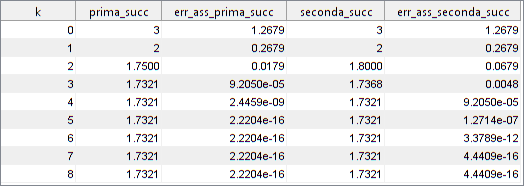
\includegraphics[scale=1]{cap1/es6.png}
\end{center}

\noindent Come si nota dalla tabella prodotta, la prima successione proposta approssima \(\sqrt3\) con un errore assoluto minore a \(10^{-12}\) (in valore assoluto) a partire dalla quinta iterazione, mentre la seconda raggiunge lo stesso risultato soltanto a partire dalla settima iterazione.
